\beginsong{Es führt über den Main}[
    wuw={Volkslied, 1952 (ergänzt und vertont von Felicitas Kuckuck, 1957)}, 
    bo={118}, 
    pfii={64}, 
    gruen={221}, 
    kssiv={80}, 
    siru={73},
    tonspur={254}, 
]

\beginverse
\endverse
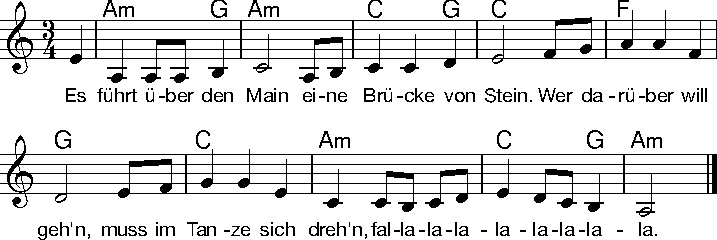
\includegraphics[draft=false, width=1\textwidth]{Noten/Lied035.pdf}	

\beginverse
Kommt ein \[Am]Fuhrmann \[G]da\[Am]her, hat ge\[C]laden \[G]gar \[C]schwer.
Seiner \[F]Rösser sind \[G]drei und sie \[C]tanzen vor\[Am]bei,
fallalala\[C]la, fala\[G]la\[Am]la.
\endverse

\beginverse
Kommt ^ein Mädchen ^al^lein auf die ^Brücke ^von ^Stein,
fasst ihr ^Röckchen ge^schwind und sie ^tanzt wie der ^Wind,
fallalala^la, fala^la^la.
\endverse

\beginverse
Kommt ^ein Bursch' oh^ne ^Schuh' und in ^Lumpen ^da^zu.
Als die ^Brücke er ^sah, hei, wie ^tanzte er ^da,
fallalala^la, fala^la^la.
\endverse

\beginverse
Und ^der König ^in Per^son, steigt he^rab von ^seinem ^Thron.
Kaum be^tritt er das ^Brett, tanzt er ^gleich Menu^ett,
fallalala^la, fala^la^la.
\endverse

\beginverse
''Lie^be Leute, ^her^bei, schlagt die ^Brücke ^ent^zwei!''
Und sie ^schwangen das ^Beil, und sie ^tanzten der^weil,
fallalala^la, fala^la^la.
\endverse

\beginverse
Al^le Leute ^im ^Land kommen ^eilig ^ge^rannt: 
''Bleibt der ^Brücke doch ^fern, denn wir ^tanzen so ^gern'',
fallalala^la, fala^la^la.
\endverse

\beginverse
Es ^führt über ^den ^Main eine ^Brücke ^von ^Stein 
und wir ^fassen die ^Händ' und wir ^tanzen ohn' ^End',
fallalala^la, fala^la^la.
\endverse

\endsong

\beginscripture{}
In dem Lied vereint die Brücke Verheißung und Bedrohung auf sich. Weil sie jeden Passanten zum Tanzen zwingt, will der König sie abreißen lassen, was jedoch von den tanzfreudigen Bürgern verhindert werden kann.
\endscripture
